% !TEX root = ./notes_template.tex
%%%%%%%%%%%%%%%%%%%%%%%%%%%%%%%%%%%%%%%%%%%%%%%%%%
%%%%%%%%%%%%%%%%%%%%% preamble %%%%%%%%%%%%%%%%%%%
%%%%%%%%%%%%%%%%%%%%%%%%%%%%%%%%%%%%%%%%%%%%%%%%%%
\documentclass[11pt,twoside]{book}


\usepackage{luatex85}


\usepackage{ctex}
\renewcommand{\contentsname}{目录}
\usepackage{fontspec}
\usepackage{xeCJK}
\setCJKmainfont{LXGW WenKai Mono}
\linespread{1.5}


\usepackage{xeCJKfntef}
\xeCJKsetup{underdot/symbol={\normalfont^^b7}}
\newcommand{\dotemph}[1]{\CJKunderdot{#1}}




%\renewcommand{\baselinestretch}{1.05}
\usepackage{amsmath,amsthm,amssymb,mathrsfs,amsfonts,dsfont}
\usepackage{epsfig,graphicx}
\usepackage{tabularx}
\usepackage{blkarray}
\usepackage{slashed}
\usepackage{color}
\usepackage{listings}
\usepackage{caption}
% \usepackage{fullpage}
\usepackage{lipsum} % provides dummy text for testing
\usepackage[toc,title,titletoc,header]{appendix}
\usepackage{minitoc}
\usepackage{color}
\usepackage{multicol} % two-col ToC
\usepackage{bm}
\usepackage{imakeidx} % before hyperref
\usepackage{hyperref}
% link colors settings
\hypersetup{
    colorlinks=true,
    citecolor=magenta,
    linkcolor=magenta,
    filecolor=green,      
    urlcolor=cyan,
    % hypertexnames=false,
}
\usepackage[capitalise]{cleveref}
\usepackage{subcaption}
\usepackage{enumitem}
\usepackage{mathtools}
\usepackage{physics}
\usepackage[linesnumbered,ruled,vlined,algosection]{algorithm2e}
\SetCommentSty{textsf}
\usepackage{epigraph}
\epigraphwidth=1.0\linewidth
\epigraphrule=0pt

% adjust margin
\usepackage[margin=2.3cm]{geometry}
\headheight13.6pt

%%%%%%%%%%%%%%%% thmtools %%%%%%%%%%%%%%%%%%%%%
\usepackage{thmtools}
\declaretheorem[numberwithin=chapter]{theorem}
\declaretheorem[numberwithin=chapter]{axiom}
\declaretheorem[numberwithin=chapter]{lemma}
\declaretheorem[numberwithin=chapter]{proposition}
\declaretheorem[numberwithin=chapter]{claim}
\declaretheorem[numberwithin=chapter]{conjecture}
\declaretheorem[sibling=theorem]{corollary}
\declaretheorem[numberwithin=chapter, style=definition]{definition}
\declaretheorem[numberwithin=chapter, style=definition]{problem}
\declaretheorem[numberwithin=chapter, style=definition]{example}
\declaretheorem[numberwithin=chapter, style=definition]{exercise}
\declaretheorem[numberwithin=chapter, style=definition]{observation}
\declaretheorem[numberwithin=chapter, style=definition]{fact}
\declaretheorem[numberwithin=chapter, style=definition]{construction}
\declaretheorem[numberwithin=chapter, style=definition]{remark}
\declaretheorem[numberwithin=chapter, style=remark]{question}
%%%%%%%%%%%%%%%% thmtools %%%%%%%%%%%%%%%%%%%%%
\usepackage{changepage}
\newenvironment{solution}
    {\renewcommand\qedsymbol{$\square$}\color{blue}\begin{adjustwidth}{0em}{2em}\begin{proof}[\textit Solution.~]}
    {\end{proof}\end{adjustwidth}}

%%%%%%%%%%%%%%%% index %%%%%%%%%%%%%%%%%%%%%
\begin{filecontents}{index.ist}
% https://tex.stackexchange.com/questions/65247/index-with-an-initial-letter-of-the-group
headings_flag 1
heading_prefix "{\\centering\\large \\textbf{"
heading_suffix "}}\\nopagebreak\n"
delim_0 "\\nobreak\\dotfill"
\end{filecontents}
\newcommand{\myindex}[1]{\index{#1} \emph{#1}}
\makeindex[columns=3, intoc, title=Alphabetical Index, options= -s index.ist]
%%%%%%%%%%%%%%%% index %%%%%%%%%%%%%%%%%%%%%

%%%%%%%%%%%%%%%% ToC %%%%%%%%%%%%%%%%%%%%%
% Link Chapter title to ToC: https://tex.stackexchange.com/questions/32495/linking-the-section-text-to-the-toc
\usepackage[explicit]{titlesec}
\titleformat{\chapter}[display]
  {\normalfont\huge\bfseries}{\chaptertitlename\ {\thechapter}}{20pt}{\hyperlink{chap-\thechapter}{\Huge#1}
\addtocontents{toc}{\protect\hypertarget{chap-\thechapter}{}}}
\titleformat{name=\chapter,numberless}
  {\normalfont\huge\bfseries}{}{-20pt}{\Huge#1}

\titleformat{\subsubsection}[runin]
  {\normalfont\large\bfseries}{}{}{#1}[]


%%%%%%%%%%%%%%%%%%% fancyhdr %%%%%%%%%%%%%%%%%
\usepackage{fancyhdr}
\pagestyle{fancy} % enable fancy page style
\renewcommand{\headrulewidth}{0.0pt} % comment if you want the rule
\fancyhf{} % clear header and footer
\fancyhead[lo,le]{\leftmark}
\fancyhead[re,ro]{\rightmark}
\fancyfoot[CE,CO]{\hyperref[toc-contents]{\thepage}}

% https://tex.stackexchange.com/questions/550520/making-each-page-number-link-back-to-beginning-of-chapter-or-section
\makeatletter
\def\chaptermark#1{\markboth{\protect\hyper@linkstart{link}{\@currentHref}{Chapter \thechapter ~ #1}\protect\hyper@linkend}{}}
\def\sectionmark#1{\markright{\protect\hyper@linkstart{link}{\@currentHref}{\thesection ~ #1}\protect\hyper@linkend}}
\makeatother
%%%%%%%%%%%%%%%%%%% fancyhdr %%%%%%%%%%%%%%%%%


%%%%%%%%%%%%%%%%%%% biblatex %%%%%%%%%%%%%%%%%
\usepackage[doi=false,url=false,isbn=false,style=alphabetic,backend=biber,backref=true, minalphanames=3]{biblatex}

\DefineBibliographyStrings{english}{
  backrefpage={Cited on page},
  backrefpages={Cited on pages}
}

\addbibresource{bib.bib}

\newbibmacro{string+doiurlisbn}[1]{%
  \iffieldundef{doi}{%
    \iffieldundef{url}{%
      \iffieldundef{isbn}{%
        \iffieldundef{issn}{%
          #1%
        }{%
          \href{http://books.google.com/books?vid=ISSN\thefield{issn}}{#1}%
        }%
      }{%
        \href{http://books.google.com/books?vid=ISBN\thefield{isbn}}{#1}%
      }%
    }{%
      \href{\thefield{url}}{#1}%
    }%
  }{%
    \href{http://dx.doi.org/\thefield{doi}}{#1}%
  }%
}

% https://tex.stackexchange.com/questions/94089/remove-quotes-from-inbook-reference-title-with-biblatex
\DeclareFieldFormat[article,incollection,inproceedings,book,misc]{title}{\usebibmacro{string+doiurlisbn}{\mkbibemph{#1}}}
% https://tex.stackexchange.com/questions/454672/biblatex-journal-name-non-italic
\DeclareFieldFormat{journaltitle}{#1\isdot}
\DeclareFieldFormat{booktitle}{#1\isdot}
% https://tex.stackexchange.com/questions/10682/suppress-in-biblatex
\renewbibmacro{in:}{}
% add video field: https://tex.stackexchange.com/questions/111846/biblatex-2-custom-fields-only-one-is-working
\DeclareSourcemap{
    \maps[datatype=bibtex]{
      \map{
        \step[fieldsource=video]
        \step[fieldset=usera,origfieldval]
    }
  }
}
\DeclareFieldFormat{usera}{\href{#1}{\textsc{Online video}}}
\AtEveryBibitem{
    \csappto{blx@bbx@\thefield{entrytype}}{% put at end of entry
        \iffieldundef{usera}{}{\space \printfield{usera}}
    }
}
%%%%%%%%%%%%%%%%%%% biblatex %%%%%%%%%%%%%%%%%

%%%%%%%%%%%%%%%%%%%%% glossaries %%%%%%%%%%%%%%%%%
% !TEX root = ./notes_template.tex
% \usepackage[style=super]{glossaries}
% https://www.overleaf.com/learn/latex/Glossaries
\usepackage[style=super,toc,acronym]{glossaries}
\setlength{\glsdescwidth}{1\linewidth}
\makeglossaries

\renewcommand\glossaryname{List of Abbreviations and Symbols}

\newglossaryentry{Q2}{name={$Q_2(f)$},
%sort=Q2,
description={Two-side (bounded) error quantum query complexity}}

\newglossaryentry{real_number}{name={$\mathbb{R}$},description={Real number}}

% \newglossaryentry{gcd}{name={gcd},description={greatest common divisor}}

\newacronym{gcd}{GCD}{Greatest Common Divisor}


\newglossaryentry{svm}{name={SVM},description={Support Vector Machine}}

\newglossaryentry{gd}{name={GD},description={Gradient Descent}}

\newglossaryentry{qft}{name={QFT},description={Quantum Field Theory}}

\newglossaryentry{qm}{name={QM},description={Quantum Mechanics}}

\newglossaryentry{v}{name={$\vec{v}$},description={a vector}}

% physics
\newglossaryentry{hamiltonian}{name={$\hat{H}$},description={Hamiltonian}}

\newglossaryentry{lagrangian}{name={$L$},description={Lagrangian}}
%%%%%%%%%%%%%%%%%%%%% glossaries %%%%%%%%%%%%%%%%%

%%%%%%%%%%%%%%%%%%%%% glossaries-extra %%%%%%%%%%%%%%%%%
% \usepackage[record,abbreviations,symbols,stylemods={list,tree,mcols}]{glossaries-extra}
%%%%%%%%%%%%%%%%%%%%% glossaries-extra %%%%%%%%%%%%%%%%%


% !TEX root = ./notes_template.tex

%%%%%%%%%%%%%%%%%%%%%%%%%%%%%%%%%%%%
%%%%%%%%%%%%%%%%%%%%%%%%%%%%%%%%%%%%
% math
\let\iff\relax
\newcommand{\iff}{\text{ iff }}
\newcommand{\OPT}{\textup{OPT}}

% physics
\newcommand{\acreation}{a^\dagger}



%%%%%%%%%%%%%%%%%%%%%%%%%%%%%%%%%%%%%%%%%%%%%%%%%%
%%%%%%%%%%%%%%%% begin of document %%%%%%%%%%%%%%%
%%%%%%%%%%%%%%%%%%%%%%%%%%%%%%%%%%%%%%%%%%%%%%%%%%

\begin{document}

\title{\bf \huge 理解 PLONK}
\author{安比实验室}
\date{\today}
\maketitle
\setcounter{tocdepth}{2}
\setcounter{minitocdepth}{1} 

% \begin{multicols}{2}
    \dominitoc% Initialization
    \adjustmtc[2]% chp number shift for mini-toc
    \tableofcontents
    \label{toc-contents}
% \end{multicols}

% 	\listoffigures
% 	% \listoftables
% \begin{multicols}{2}
% 	\listoftheorems[ignoreall,show={theorem}]
% \end{multicols}

% 	\renewcommand{\listtheoremname}{List of Definitions}
% \begin{multicols}{2}
% 	\listoftheorems[ignoreall,show={definition}]
% \end{multicols}

	% \printglossaries
	% \printglossary[type=\acronymtype]
	% \printglossary
	% \printglossary[title=List of terms, toctitle=List of terms]

	% bib2gls
	% \printunsrtglossaries % print all types
	% \printunsrtglossary[type={abbreviations},title=List of Abbreviations,style=listgroup]
	% \printunsrtglossary[type={abbreviations},title=List of Abbreviations,style=listhypergroup] % doesn't work
	% \printunsrtglossary[type={symbols},title=List of Symbols,style=listgroup]
	% \printunsrtglossary % main entry

%%%%%%%%%%%%%%%Content%%%%%%%%%%%%%%%
% \mainmatter % separat the number of toc and mainmatter
% 原始模版内容
% \input{./chapter/preface.tex}

% \part{Mathematics}
% \input{./chapter/discrete_math.tex}

% \part{Computer Science}
% % \input{./chapter/complexity.tex}
% \input{./chapter/machine_learning.tex}
% % \input{./chapter/algorithms.tex}

% \part{Physics}
% \input{./chapter/quantum_mechanics.tex}
% % \input{./chapter/quantum_field_theory.tex}

% \begin{appendices}
%   \input{./chapter/appendix_formula.tex}
%   \end{appendices}


\section{理解 PLONK(一):Plonkish
Arithmetization}\label{ux7406ux89e3-plonkux4e00plonkish-arithmetization}

算术化是指把计算转换成数学对象,然后进行零知识证明。 Plonkish 算术化是
Plonk 证明系统特有的算术化方法,在 Plonkish
出现之前,主流的电路表达形式为 R1CS,被 Pinocchio,Groth16,Bulletproofs
等广泛采用。2019 年 Plonk 方案提出了一种看似复古的电路编码方式,但由于
Plonk
方案将多项式的编码应用到了极致,它不再局限于算术电路中的「加法门」和「乘法门」,而是可以支持更灵活的「自定义门」与「查表门」。

我们先回顾一下 R1CS
的电路编码,也是相关介绍最多的算术化方案。然后我们对比引入 Plonkish
编码。

\hypertarget{ux7b97ux672fux7535ux8defux4e0e-r1cs-ux7b97ux672fux5316}{%
\subsection{算术电路与 R1CS
算术化}\label{ux7b97ux672fux7535ux8defux4e0e-r1cs-ux7b97ux672fux5316}}

一个算术电路包含若干个乘法门与加法门。每一个门都有「两个输入」引脚和一个「输出」引脚,任何一个输出引脚可以被接驳到多个门的输入引脚上。

先看一个非常简单的算术电路:

\begin{figure}
\centering
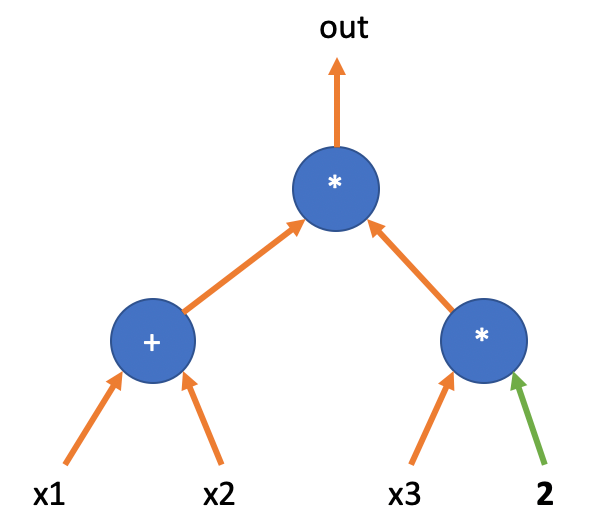
\includegraphics{img/img20230414162317.png}
\caption{img20230414162317}
\end{figure}

这个电路表示了这样的一个计算:

\[
(x_1 + x_2) \cdot (2\cdot x_3) = out
\]

电路中有4个变量,其中三个变量为输入变量 \((x_1, x_2, x_3)\)
,一个输出变量 \(out\),其中还有一个输入为常数,其值为 \(2\)。

一个电路有两种状态:「空白态」和「运算态」。当输入变量没有具体值的时候,电路处于「空白态」,这时我们只能描述电路引线之间的关系,即电路的结构拓扑。

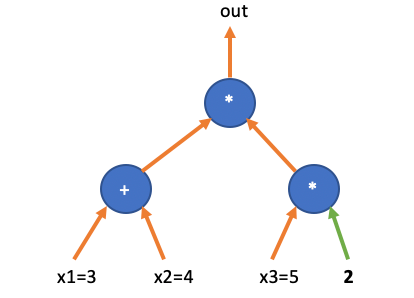
\includegraphics{img/img20230414162845.png}

接下来的问题是,我们要先编码电路的「空白态」,即编码各个门的位置,和他们之间引线连接关系。

R1CS
是通过图中的乘法门为中心,用三个「选择子」矩阵来「选择」乘法门的「左输入」、「右输入」、「输出」都分别连接了那些变量。

我们先看看图中最上面的乘法门的左输入,可以用下面的表格来描述:

\[
\begin{array}{|c|c|c|c|c|}
\hline
1 & x_1 & x_2 & x_3 & out \\
\hline
0 & 1 & 1 & 0 & 0 \\
\hline
\end{array}
\]

这个表格只有一行,因此我们可以用一个向量 \(U=(0,1,1,0,0)\)
来代替,表示乘法门的左输入连接了两个变量,\(x1\) 和
\(x_2\)。记住,所有的加法门都会被展开成多个变量的相加(或线性组合)。

再看看其右输入,连接了一个变量 \(x_3\) 和一个常数值,等价于连接了
\(x_3\) 的两倍,那么右输入的选择子矩阵可以记为

\[
\begin{array}{|c|c|c|c|c|}
\hline
1 & x_1 & x_2 & x_3 & out \\
\hline
0 & 0 & 0 & 2 & 0 \\
\hline
\end{array}
\]

这里同样可以用一个行向量 \(V=(0,0,0,2,0)\) 来表示,其中的 \(2\)
即为上图中电路的常数引线。

最后乘法门的输出按照上面的方法可以描述为 \(W=(0,0,0,0,1)\),即输出变量为
\(out\):

\[
\begin{array}{|c|c|c|c|c|}
\hline
1 & x_1 & x_2 & x_3 & out \\
\hline
0 & 0 & 0 & 0 & 1 \\
\hline
\end{array}
\]

有了三个向量 \((U,V,W)\),我们可以通过一个「内积」等式来约束电路的运算:

\[
\big(U\cdot(1,x_1, x_2,x_3,out)\big) \cdot \big(V\cdot(1,x_1, x_2,x_3,out)\big) = \big(W\cdot(1,x_1, x_2,x_3,out)\big)
\]

这个等式化简之后正好可以得到:

\[
(x_1 + x2) \cdot (2\cdot x_3) = out
\]

如果我们把这几个变量换成赋值向量
\((1,x_1,x_2,x_3,out) = (1,3,4,5,70)\),那么电路的运算可以通过「内积」等式来验证:

\[
(U\cdot(1,3,4,5,70))\cdot(U\cdot(1,3,4,5,70))=W\cdot(1,3,4,5,70)
\]

而一个错误的赋值向量,比如 \((1,3,4,\fbox{0},70)\)
,则不满足「内积等式」:

\[
(U\cdot(1,3,4,\fbox{0},70))\cdot(U\cdot(1,3,4,\fbox{0},70))\neq W\cdot(1,3,4,\fbox{0},70)
\]

左边运算结果为 \(0\),右边运算结果为 \(70\)。当然,我们可以验证
\((1,3,4,0,0)\) 也是一组合法(满足电路约束)的赋值。

并不是任何一个电路都存在赋值向量。凡是存在合法的赋值向量的电路,被称为可被满足的电路。判断一个电路是否可被满足,是一个
NP-Complete 问题,也是一个 NP 困难问题。

这里例子中的两个乘法门并不相同,上面的乘法门是左右输入中都含有变量,而下面的乘法门只有一边的输入为变量,另一边为常数。对于后者这类「常数乘法门」,后续我们也把他们看作为特殊的「加法门」,如下图所示,左边电路右下的乘法门等价于右边电路的右下加法门。

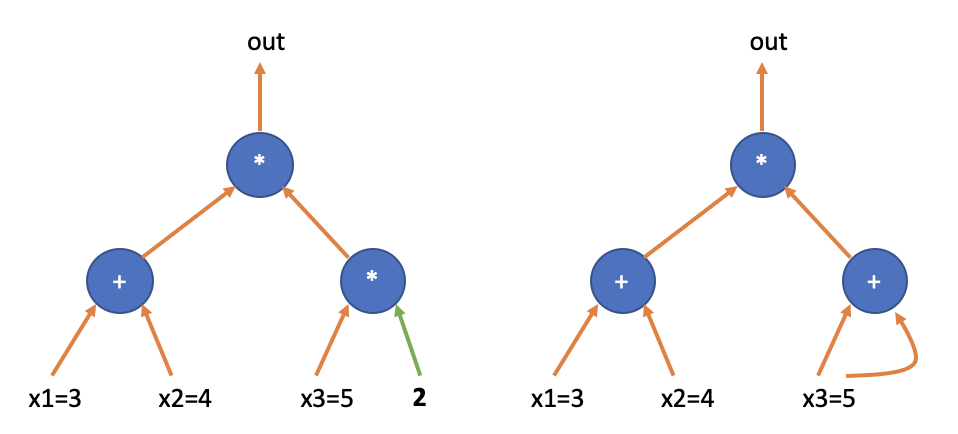
\includegraphics{img/img20230423133455.png}

那么如果一个电路含有两个以上的乘法门,我们就不能用 \(U,V,W\)
三个向量之间的内积关系来表示运算,而需要构造「三个矩阵」的运算关系。

\hypertarget{ux591aux4e2aux4e58ux6cd5ux95e8}{%
\subsubsection{多个乘法门}\label{ux591aux4e2aux4e58ux6cd5ux95e8}}

比如下图所示电路,有两个乘法门,他们的左右输入都涉及到变量。

% \includegraphics{img/img20230414170601.png}

这个电路表示了这样的一个计算:

\[
(x_1 + x2) \cdot (x3 \cdot x4) = out
\]

我们以\textbf{乘法门}为基准,对电路进行编码。第一步将电路中的乘法门依次编号(无所谓编码顺序,只要前后保持一致)。图中的两个乘法门编码为
\texttt{\#1} 与 \texttt{\#2}。

然后我们需要为每一个乘法门的中间值引线也给出变量名:比如四个输入变量被记为
\(x_1, x_2, x_3, x_4\),其中 \(x_5\)
为第二个乘法门的输出,同时作为第一个乘法门的右输入。而 \(out\)
为第一个乘法门的输出。于是我们可以得到一个关于变量名的向量:

\[
(x_1, x_2, x_3, x_4, x_5, out)
\]

该电路的「空白态」可以用下面的三个矩阵来编码:

\[
U, V, W \in \mathbb{F}^{n\times m}
\]

其中 \(n\) 为乘法门的数量,而 \(m\) 大致为引线的数量。每一个矩阵的第
\(i\) 行「选择」了第 \(i\)
个乘法门的输入输出变量。比如我们定义电路的左输入矩阵 \(U\) :

% \[
% \begin{array}{|c|c|c|c|c|}
% \hline
% x_1 & x_2 & x_3 & x_4 & x_5 & out & \texttt{i} \\
% \hline
% 1 & 1 & 0 & 0 & 0 & 0 & \texttt{1}\\
% \hline
% 0 & 0 & 1 & 0 & 0 & 0 & \texttt{2}\\
% \hline
% \end{array}
% \]

% 其中第一个乘法门的左输入为 \((x_1+x_2)\), 第二个乘法门的左输入为
% \(x_3\)。右输入矩阵 \(V\) 定义为:

% \[
% \begin{array}{|c|c|c|c|c|}
% \hline
% x_1 & x_2 & x_3 & x_4 & x_5 & out &\texttt{i}\\
% \hline
% 0 & 0 & 0 & 0 & 1 & 0 & \texttt{1}\\
% \hline
% 0 & 0 & 0 & 1 & 0 & 0 & \texttt{2}\\
% \hline
% \end{array}
% \]

% 其中1号门的右输入为 \(x_5\),第二个乘法门的右输入为
% \(x_4\)。最后定义输出矩阵 \(W\):

% \[
% \begin{array}{|c|c|c|c|c|}
% \hline
% x_1 & x_2 & x_3 & x_4 & x_5 & out & \texttt{i}\\
% \hline
% 0 & 0 & 0 & 0 & 0 & 1 & \texttt{1}\\
% \hline
% 0 & 0 & 0 & 0 & 1 & 0 & \texttt{2}\\
% \hline
% \end{array}
% \]

我们把所有的引线赋值看作为一个向量: \(\vec{a}\) (这里用字母
\(a\),取自 Assignments 首字母)

在上面的例子中,「赋值向量」为

\[
\vec{a} = (x_1, x_2, x_3,x_4,x_5,out)
\]

于是我们可以轻易地检验下面的等式

\[
(U \cdot \vec{a}) \circ (V \cdot \vec{a}) = (W \cdot\vec{a})
\]

其中符号 \(\circ\) 为 Hadamard
Product,表示「按位乘法」。展开上面的按位乘法等式,我们可以得到这个电路的运算过程:

\[
\left[
\begin{array}{c}
x_1 + x_2 \\
x_3 \\
\end{array}
\right]
\circ
\left[
\begin{array}{c}
x_5 \\
x_4 \\
\end{array}
\right]=
\left[
\begin{array}{c}
out \\
x_5 \\
\end{array}
\right]
\]

请注意,通常「赋值向量」中需要一个固定赋值为 \(1\)
的变量,这是为了处理加法门中的常量输入。

\hypertarget{ux4f18ux7f3aux70b9}{%
\subsubsection{优缺点}\label{ux4f18ux7f3aux70b9}}

由于 R1CS 编码以乘法门为中心,于是电路中的加法门并不会增加 \(U, V, W\)
矩阵的行数,因而对 Prover 的性能影响不大。R1CS
电路的编码清晰简单,利于在其上构造各种 SNARK 方案。

在 2019 年 Plonk
论文中的编码方案同时需要编码加法门与乘法门,看起来因此会增加约束的数量,降低
Proving 性能。但 Plonk
团队随后陆续引入了除乘法与加法外的运算门,比如实现范围检查的门,实现异或运算的门等等。不仅如此,Plonk
支持任何其输入输出满足多项式关系的门,即 Custom Gate,还有适用于实现 RAM
的状态转换门等,随着查表门的提出,Plonk
方案逐步成为许多应用的首选方案,其编码方式也有了一个专门的名词:Plonkish。

\hypertarget{plonkish-ux7b97ux672fux95e8}{%
\subsection{Plonkish 算术门}\label{plonkish-ux7b97ux672fux95e8}}

回看下例子电路,我们把三个门全都编号,
\(\texttt{1},\texttt{2},\texttt{3}\),同时把加法门的输出值也标记为变量
\(x_6\)。

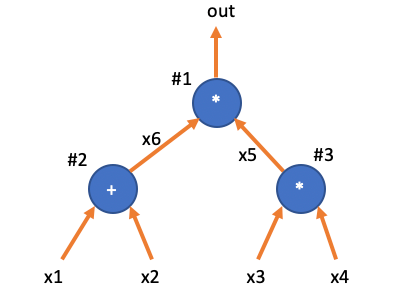
\includegraphics{img/img20230414202348.png}
显然,上面的电路满足三个约束:

% \begin{itemize}
% \tightlist
% \item
%   \(x_1 + x_2 =x_6\)
% \item
%   \(x_3\cdot x_4 = x_5\)
% \item
%   \(x_6 \cdot x_5 = out\)
% \end{itemize}

我们定义一个矩阵 \(W\in\mathbb{F}^{n\times 3}\) 来表示约束( \(n\)
为算术门的数量):

\[
\begin{array}{c|c|c|c|}
\texttt{i} & w_a & w_b & w_c  \\
\hline
\texttt{1} & x_6 & x_5 & out \\
\texttt{2} & x_1 & x_2 & x_6 \\
\texttt{3} & x_3 & x_4 & x_5 \\
\end{array}
\]

为了区分加法和乘法,我们再定一个向量 \(Q\in\mathbb{F}^{n\times5}\)
来表示运算符

% \[
% \begin{array}{c|c|c|c|}
% \texttt{i}  & q_L & q_R & q_M & q_C & q_O  \\
% \hline
% \texttt{1} & 0 & 0 & 1 & 0& 1 \\
% \texttt{2} & 1 & 1 & 0 & 0& 1 \\
% \texttt{3} & 0 & 0 & 1 & 0& 1 \\
% \end{array}
% \]

于是我们可以通过下面的等式来表示三个约束:

\[
q_L \circ w_a + q_R \circ w_b + q_M\circ(w_a\cdot w_b) + q_C -  q_O\circ w_c = 0
\]

如果把上面的等式代入并展开,我们可以得到下面的约束等式:

\[
\left[
\begin{array}{c}
0\\
1 \\
0\\
\end{array}
\right]
\circ
\left[
\begin{array}{c}
x_6 \\
x_1 \\
x_5\\
\end{array}
\right]
+
\left[
\begin{array}{c}
0\\
1 \\
0\\
\end{array}
\right]
\circ
\left[
\begin{array}{c}
x_5 \\
x_2 \\
x_4\\
\end{array}
\right]
+
\left[
\begin{array}{c}
1\\
0 \\
1\\
\end{array}
\right]
\circ
\left[
\begin{array}{c}
x_6\cdot x_5 \\
x_1\cdot x_2 \\
x_3\cdot x_4\\
\end{array}
\right]=\left[
\begin{array}{c}
1\\
1 \\
1\\
\end{array}
\right]
\circ
\left[
\begin{array}{c}
out \\
x_6 \\
x_5\\
\end{array}
\right]
\]

化简后得:

\[
\left[
\begin{array}{c}
0 \\
x_1 \\
0\\
\end{array}
\right]
+
\left[
\begin{array}{c}
0 \\
x_2 \\
0\\
\end{array}
\right]
+
\left[
\begin{array}{c}
x_6\cdot x_5 \\
0 \\
x_3\cdot x_4\\
\end{array}
\right]=\left[
\begin{array}{c}
out \\
x_6 \\
x_5\\
\end{array}
\right]
\]

这正好是三个算术门的计算约束。

总结下,Plonkish 需要一个矩阵 \(Q\)
来描述电路空白态,而所有的赋值则写入了 \(W\) 矩阵。对于 Prover 和
Verifier 的交换协议,\(W\) 是 Prover 的 witness,属于秘密知识,对
Verifier 保密, \(Q\) 矩阵代表了一个实现双方约定共识的电路描述。

不过仅仅有 \(Q\) 矩阵是不足以精确描述上面的例子电路。

\hypertarget{ux590dux5236ux7ea6ux675f}{%
\subsection{复制约束}\label{ux590dux5236ux7ea6ux675f}}

比较下面两个电路,它们的 \(Q\) 矩阵完全相同,但它们却完全不同。

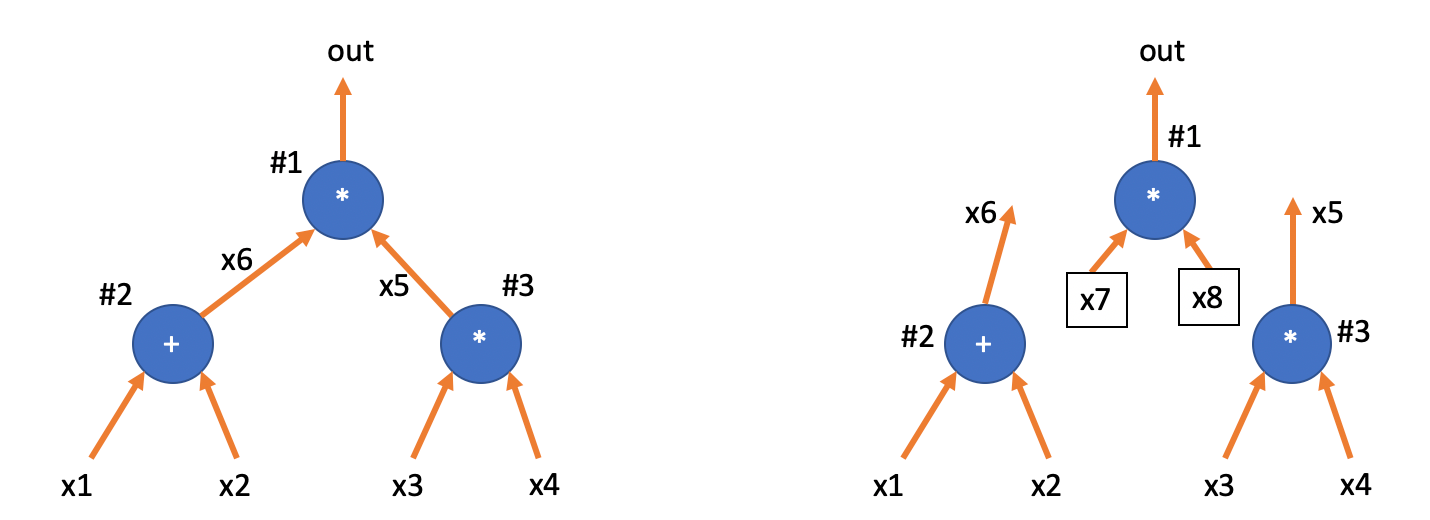
\includegraphics{img/img20230414205219.png}

两个电路的区别在于 \(x_5, x_6\) 是否被接入了 \texttt{\#1} 号门。如果让
Prover 直接把电路赋值填入 \(W\) 表格,一个「诚实的」Prover 会在
\(w_{a,1}\) 和 \(w_{c,2}\) 两个位置填上相同的值;而一个「恶意的」Prover
完全可以填上不同的值。如果恶意 Prover 在 \(w_{b,1}\) 和 \(w_{c,3}\)
也填入不同的值,那么实际上 Prover 证明的是上图右边的电路,而非是和
Verifier 共识过的电路(左边)。

% \[
% \begin{array}{c|c|c|c|}
% i & w_a & w_b & w_c  \\
% \hline
% 1 & \boxed{x_6} & \underline{x_5} & out \\
% 2 & x_1 & x_2 & \boxed{x_6} \\
% 3 & x_3 & x_4 & \underline{x_5} \\
% \end{array}
% \]

我们需要增加新的约束,强制要求右边电路图中 \(x_6=x_7\) 和
\(x_5=x_8\)。这等价于我们要求 Prover
把同一个变量填入表格多个位置时,\textbf{必须填入相等的值}。

这就需要一类新的约束------「拷贝约束」,即 Copy Contraint。Plonk
采用「置换证明」保证 \(W\)
表格中多个位置上的值满足拷贝关系。我们继续用上面这个电路图的案例来说明其基本思路:

设想我们把 \(W\) 表格中的所有位置索引排成一个向量:

\[
\sigma_0=(\boxed{w_{a,1}}, w_{a,2}, w_{a,3}, \underline{w_{b,1}}, w_{b,2}, w_{b,3}, w_{c,1}, \boxed{w_{c,2}}, \underline{w_{c,3}})
\]

然后把应该相等的两个位置互换,比如上图中要求 \(w_{a,1}=w_{c,2}\) 和
\(w_{b,1}=w_{c,3}\) 。于是我们得到了下面的位置向量:

\[
\sigma=(\boxed{w_{c,2}}, w_{a,2}, w_{a,3}, \underline{w_{c,3}}, w_{b,2}, w_{b,3}, w_{c,1}, \boxed{w_{a,1}}, \underline{w_{b,1}})
\]

然后我们要求 Prover 证明:\textbf{\(W\)
表格按照上面的置换之后,仍然等于自身}。置换前后的相等性可以保证 Prover
无法作弊。

再来一个例子,当约束一个向量中有三个(或多个)位置上的值必须相同时,只需要把这三个(或多个)位置的值进行循环移位(左移位或者右移位),然后证明移位后的向量与原向量相等即可。比如:

\[
A = (b_1, b_2, \underline{a_1}, b_3, \underline{a_2}, b_4, \underline{a_3})
\]

如果要证明 \(a_1=a_2=a_3\),那么只需要证明:

\[
A' =  (b_1, b_2, \underline{a_3}, b_3, \underline{a_1}, b_2, \underline{a_2}) \overset{?}{=} A
\]

在经过置换的向量 \(A'\) 中, \(a_1, a_2, a_3\) 依次右移交换,即 \(a_1\)
放到了原来 \(a_2\) 的位置,而 \(a_2\) 放到了 \(a_3\) 的位置, \(a_3\)
则放到了 \(a_1\) 的位置。

如果 \(A'=A\) ,那么 \(A'\) 和 \(A\)
所有对应位置上的值都应该相等,可得: \(a_1=a_4\), \(a_2=a_1\),
\(a_3=a_2\),即
\(a_1=a_2=a_3\)。这个方法可以适用于任意数量的等价关系。(后续证明两个向量相等的方法请见下章)

那么如何描述电路赋值表格中的交换呢?我们只需要记录 \(\sigma\)
向量即可,当然 \(\sigma\) 向量也可以写成表格的形式:

\[
\begin{array}{c|c|c|c|}
i & \sigma_a & \sigma_b & \sigma_c  \\
\hline
1 & \boxed{w_{c,2}} & \underline{w_{c,3}}& w_{c,1} \\
2 & w_{a,2} & w_{b,2} & \boxed{w_{a,1}} \\
3 & w_{a,3} & w_{b,3} & \underline{w_{b,1}} \\
\end{array}
\]

加上 \(\sigma\) ,空白电路可以描述为 \((Q,\sigma)\) ,电路的赋值为 \(W\)

\[
\mathsf{Plonkish}_0 \triangleq (Q, \sigma; W)
\]

\hypertarget{ux518dux6bd4ux8f83}{%
\subsection{再比较}\label{ux518dux6bd4ux8f83}}

R1CS 的 \((U,V,W)\)
表格的宽度与引线的数量有关,行数跟乘法门数量有关。这个构造相当于把算术电路看成是仅有乘法门构成,但每个门有多个输入引脚(最多为所有引线的数量)。而
Plonkish 则是同等对待加法门与乘法门,并且因为输入引脚只有两个, 所以
\(W\)
表格的宽度固定,仅有三列(如果要支持高级的计算门,表格可以扩展到更多列)。这一特性是
Plonk 可以利用 Permutation Argument 实现拷贝约束的前提。

\begin{quote}
\ldots, and thus our linear contraints are just wiring constraints that
can be reduced to a permutation check.
\end{quote}

按照 Plonk
论文的统计,一般情况下,算术电路中加法门的数量是乘法门的两倍。如果这样看来,
\(W\) 表格的长度会三倍于 R1CS
的矩阵。但这个让步会带来更多的算术化灵活度。

\hypertarget{ux7535ux8defux9a8cux8bc1ux534fux8baeux6846ux67b6}{%
\subsection{电路验证协议框架}\label{ux7535ux8defux9a8cux8bc1ux534fux8baeux6846ux67b6}}

有了电路空白结构的描述和赋值,我们可以大致描述下 Plonk 的协议框架。

首先 Prover 和 Verifier 会对一个共同的电路进行共识, \((Q,\sigma)\) 。
假设电路的公开输出为 \(out=99\),而 \((x_1,x_2,x_3,x_4)\) 为秘密输入。

Prover 填写 \(W\) 矩阵(Verifier 不可见):

\[
\begin{array}{c|c|c|c|}
i & w_a & w_b & w_c  \\
\hline
1 & \boxed{x_6} & \underline{x_5} & [out] \\
2 & x_1 & x_2 & \boxed{x_6} \\
3 & x_3 & x_4 & \underline{x_5} \\
4 & 0 & 0 & [out] \\
\end{array}
\]

其中增加的第四行是为了增加一个额外的算术约束: \(out=99\) ,把 \(out\)
值显示地表示在 \(Q\) 矩阵中。

相应的那么 Prover 和 Verifier 共识的 \(Q\) 矩阵为

% \[
% \begin{array}{c|c|c|c|}
% i & q_L & q_R & q_M & q_C & q_O  \\
% \hline
% 1 & 0 & 0 & 1 & 0& 1 \\
% 2 & 1 & 1 & 0 & 0& 1 \\
% 3 & 0 & 0 & 1 & 0& 1 \\
% 4 & 0 & 0 & 0 & 99& 1 \\
% \end{array}
% \]

其中第四行约束,保证 \(out=99\),可以把
\((q_L=0, q_R=0,q_M=0,q_C=99,q_O=1)\) 代入下面的算术约束,可得
\(99-w_c = 0\) ,即 \(w_{c,4}=99\) 。

\[
q_L \circ w_a + q_R \circ w_b + q_M\circ(w_a\cdot w_b) + q_C -  q_O\circ w_c = 0
\]

为了保证第一行的 \(w_c\) 也必须为 \(99\),这就需要在 \(\sigma\)
矩阵中添加额外的一条拷贝约束:让 \(out\) 变量的位置 \((w_{c,1})\) 与
第四行的输出 \(w_{c,4}\) 交换对调:

\[
\begin{array}{c|c|c|c|}
i & \sigma_a & \sigma_b & \sigma_c  \\
\hline
1 & \boxed{w_{c,2}} & \underline{w_{c,3}} & [w_{c,4}] \\
2 & w_{a,2} & w_{b,2} & \boxed{w_{a,1}} \\
3 & w_{a,3} & w_{b,3} & \underline{w_{b,1}} \\
4 & w_{a,4} & w_{b,4} & [w_{c,1}]\\
\end{array}
\]

如果 Prover 是诚实的,那么对于
\(i\in(1,2,3,4)\),下面的算术约束等式成立:

\[
q_{L,i} \circ w_{a,i} + q_{R,i} \circ w_{b,i} + q_{M,i}\circ(w_{a,i}\cdot w_{b,i}) + q_{C,i} -  q_{O,i}\circ w_{c,i} = 0
\]

验证协议的大概思路如下:

协议开始:Prover 如实填写 \(W\) 表格,然后把 \(W\)
表格的每一列进行编码,并进行多项式编码,并把编码后的结果发送给 Verifier

协议验证阶段:Verifier 与 Prover
通过进一步的交互,验证下面的等式是否成立:

\[
q_{L}(X) \cdot w_{a}(X) + q_{R}(X) \cdot w_{b}(X) + q_{M}(X)\cdot(w_{a}(X)\cdot w_{b}(X)) + q_{C}(X) -  q_{O}(X)\cdot w_{c}(X) \overset{?}{=} 0
\]

当然这个验证还不够,还要验证 \((\sigma_a(X),\sigma_b(X),\sigma_c(X))\)
与 \((w_a(X),w_b(X),w_c(X))\) 之间的关系。还有,Verifier
如何通过多项式来验证电路的运算,请看后续章节。

% \hypertarget{ux53c2ux8003ux6587ux732e}{%
% \subsection{参考文献}\label{ux53c2ux8003ux6587ux732e}}

% \begin{itemize}
% \tightlist
% \item
%   {[}BG12{]} Bayer, Stephanie, and Jens Groth. ``Efficient
%   zero-knowledge argument for correctness of a shuffle.'' \emph{Annual
%   International Conference on the Theory and Applications of
%   Cryptographic Techniques}. Springer, Berlin, Heidelberg, 2012.
% \item
%   {[}GWC19{]} Ariel Gabizon, Zachary J. Williamson, and Oana Ciobotaru.
%   ``Plonk: Permutations over lagrange-bases for oecumenical
%   noninteractive arguments of knowledge.'' \emph{Cryptology ePrint
%   Archive} (2019).
% \end{itemize}



% \input{./chapter/02Randomness.tex}
% \input{./chapter/03Definition.tex}
% \input{./chapter/04IP.tex}
% \input{./chapter/05FS.tex}
% \input{./chapter/06FrontEnds.tex}
% \input{./chapter/07argfromip.tex}
% \input{./chapter/08MIP.tex}
% \input{./chapter/09PCP.tex}
% \input{./chapter/10IOP.tex}
% \input{./chapter/11ZKP.tex}
% \input{./chapter/12sigma.tex}
% \input{./chapter/13CP.tex}
% \input{./chapter/14PCDL.tex}
% \input{./chapter/15PCPairing.tex}
% \input{./chapter/16PC.tex}
% \input{./chapter/17LPCP.tex}
% \input{./chapter/18Recursion.tex}
% \input{./chapter/19SNARK.tex}



\backmatter

%%%%%%%%%%%%%%% Reference %%%%%%%%%%%%%%%

\printbibliography[heading=bibintoc]
\printindex

\end{document}

